\begin{figure}[ht]
  \centering
  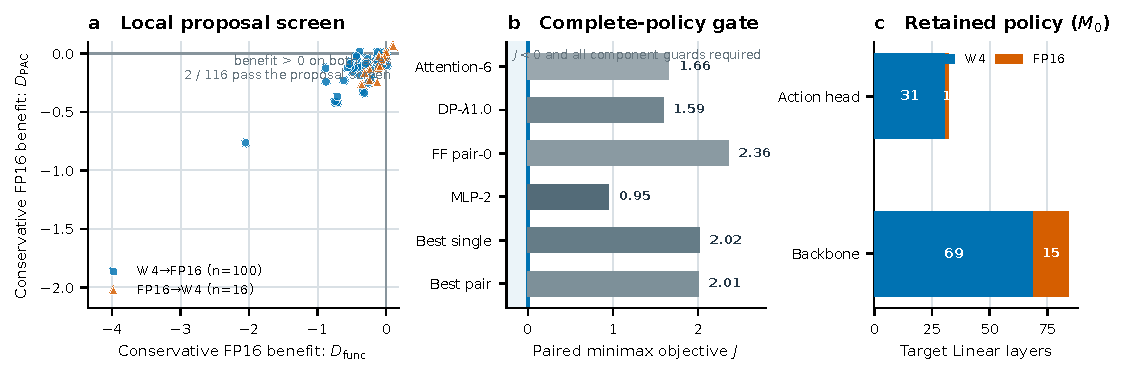
\includegraphics[width=\textwidth]{figures/dypac_fcp_audit.pdf}
  \caption{GR00T deviation-based decision record with corrected task-level statistics. \textbf{(a)} Two of 116 coordinates have positive conservative benefit for retaining FP16 under both metrics. Both are already protected; these are not two improving removals. \textbf{(b)} All six rebuilt complete-policy candidates have $J>0$ and fail a component guard. \textbf{(c)} The 100-W4/16-FP16 initializer is retained. This decision does not establish its success optimality or demonstrate an effect of candidate-state adjudication, which was not triggered.}
  \label{fig:fcp_audit}
\end{figure}